\documentclass[]{book}
\usepackage{lmodern}
\usepackage{amssymb,amsmath}
\usepackage{ifxetex,ifluatex}
\usepackage{fixltx2e} % provides \textsubscript
\ifnum 0\ifxetex 1\fi\ifluatex 1\fi=0 % if pdftex
  \usepackage[T1]{fontenc}
  \usepackage[utf8]{inputenc}
\else % if luatex or xelatex
  \ifxetex
    \usepackage{mathspec}
  \else
    \usepackage{fontspec}
  \fi
  \defaultfontfeatures{Ligatures=TeX,Scale=MatchLowercase}
\fi
% use upquote if available, for straight quotes in verbatim environments
\IfFileExists{upquote.sty}{\usepackage{upquote}}{}
% use microtype if available
\IfFileExists{microtype.sty}{%
\usepackage{microtype}
\UseMicrotypeSet[protrusion]{basicmath} % disable protrusion for tt fonts
}{}
\usepackage[margin=1in]{geometry}
\usepackage{hyperref}
\hypersetup{unicode=true,
            pdftitle={Brisbane Birds},
            pdfborder={0 0 0},
            breaklinks=true}
\urlstyle{same}  % don't use monospace font for urls
\usepackage{longtable,booktabs}
\usepackage{graphicx,grffile}
\makeatletter
\def\maxwidth{\ifdim\Gin@nat@width>\linewidth\linewidth\else\Gin@nat@width\fi}
\def\maxheight{\ifdim\Gin@nat@height>\textheight\textheight\else\Gin@nat@height\fi}
\makeatother
% Scale images if necessary, so that they will not overflow the page
% margins by default, and it is still possible to overwrite the defaults
% using explicit options in \includegraphics[width, height, ...]{}
\setkeys{Gin}{width=\maxwidth,height=\maxheight,keepaspectratio}
\IfFileExists{parskip.sty}{%
\usepackage{parskip}
}{% else
\setlength{\parindent}{0pt}
\setlength{\parskip}{6pt plus 2pt minus 1pt}
}
\setlength{\emergencystretch}{3em}  % prevent overfull lines
\providecommand{\tightlist}{%
  \setlength{\itemsep}{0pt}\setlength{\parskip}{0pt}}
\setcounter{secnumdepth}{5}
% Redefines (sub)paragraphs to behave more like sections
\ifx\paragraph\undefined\else
\let\oldparagraph\paragraph
\renewcommand{\paragraph}[1]{\oldparagraph{#1}\mbox{}}
\fi
\ifx\subparagraph\undefined\else
\let\oldsubparagraph\subparagraph
\renewcommand{\subparagraph}[1]{\oldsubparagraph{#1}\mbox{}}
\fi

%%% Use protect on footnotes to avoid problems with footnotes in titles
\let\rmarkdownfootnote\footnote%
\def\footnote{\protect\rmarkdownfootnote}

%%% Change title format to be more compact
\usepackage{titling}

% Create subtitle command for use in maketitle
\newcommand{\subtitle}[1]{
  \posttitle{
    \begin{center}\large#1\end{center}
    }
}

\setlength{\droptitle}{-2em}
  \title{Brisbane Birds}
  \pretitle{\vspace{\droptitle}\centering\huge}
  \posttitle{\par}
  \author{Richard A. Fuller\(^1\), Jeffrey O. Hanson\(^1\)\\
\(^1\)School of Biological Sciences, The University of Queensland,
Brisbane, QLD, Australia\\
Correspondance should be addressed to
\href{mailto:r.fuller@uq.edu.au}{\nolinkurl{r.fuller@uq.edu.au}}}
  \preauthor{\centering\large\emph}
  \postauthor{\par}
  \date{}
  \predate{}\postdate{}

% load packages
\usepackage{amsmath,amsfonts,float,makecell,hyperref}
\usepackage[T1]{fontenc}
\usepackage{lmodern}
\usepackage[utf8]{inputenc}
\usepackage[doublespacing]{setspace}

% format captions
\usepackage[labelfont={small,bf}, labelsep=space, font={small}]{caption}

% allow breaks in equations
\allowdisplaybreaks

% make figures static
\let\origfigure\figure
\let\endorigfigure\endfigure
\renewenvironment{figure}[1][2] {
  \expandafter\origfigure\expandafter[H]
} {
  \endorigfigure
}

\begin{document}
\maketitle

{
\setcounter{tocdepth}{1}
\tableofcontents
}
\chapter{Preface}\label{preface}

Lorem ipsum dolor sit amet, consectetur adipiscing elit. Donec sed justo
nunc. In in cursus turpis, sollicitudin pellentesque lacus. Aliquam et
orci malesuada, tristique justo quis, feugiat ex. Phasellus at sem sit
amet sapien consequat fringilla. Praesent pretium aliquet ante, eu
maximus augue placerat ut. Donec odio erat, vehicula non accumsan quis,
ultricies eu arcu. Aliquam erat volutpat.

In hac habitasse platea dictumst. Nullam lacus elit, luctus a cursus ut,
tempus id arcu. Quisque ornare eleifend augue, ac aliquet sapien posuere
porttitor. Nam lacinia, diam at molestie tempor, erat ligula vulputate
ligula, id rutrum magna justo in lorem. Vivamus posuere risus augue. Ut
velit elit, hendrerit sit amet lacus nec, mattis commodo neque. Cras vel
felis sed purus sollicitudin pharetra eu eget arcu. In volutpat eleifend
mauris, sed porta nunc dapibus a. Suspendisse fringilla tempus quam a
fermentum. Morbi quis lacus nec eros maximus interdum. Nullam venenatis
vehicula magna, a egestas est ornare vel. Fusce quis luctus orci, eget
congue dolor. Morbi luctus est justo, quis porttitor lacus facilisis sit
amet.

\chapter{\texorpdfstring{Honeyeaters and Chats
\emph{Meliphagidae}}{Honeyeaters and Chats Meliphagidae}}\label{honeyeaters-and-chats-meliphagidae}

Lorem ipsum dolor sit amet, consectetur adipiscing elit. Donec sed justo
nunc. In in cursus turpis, sollicitudin pellentesque lacus. Aliquam et
orci malesuada, tristique justo quis, feugiat ex. Phasellus at sem sit
amet sapien consequat fringilla. Praesent pretium aliquet ante, eu
maximus augue placerat ut. Donec odio erat, vehicula non accumsan quis,
ultricies eu arcu. Aliquam erat volutpat.

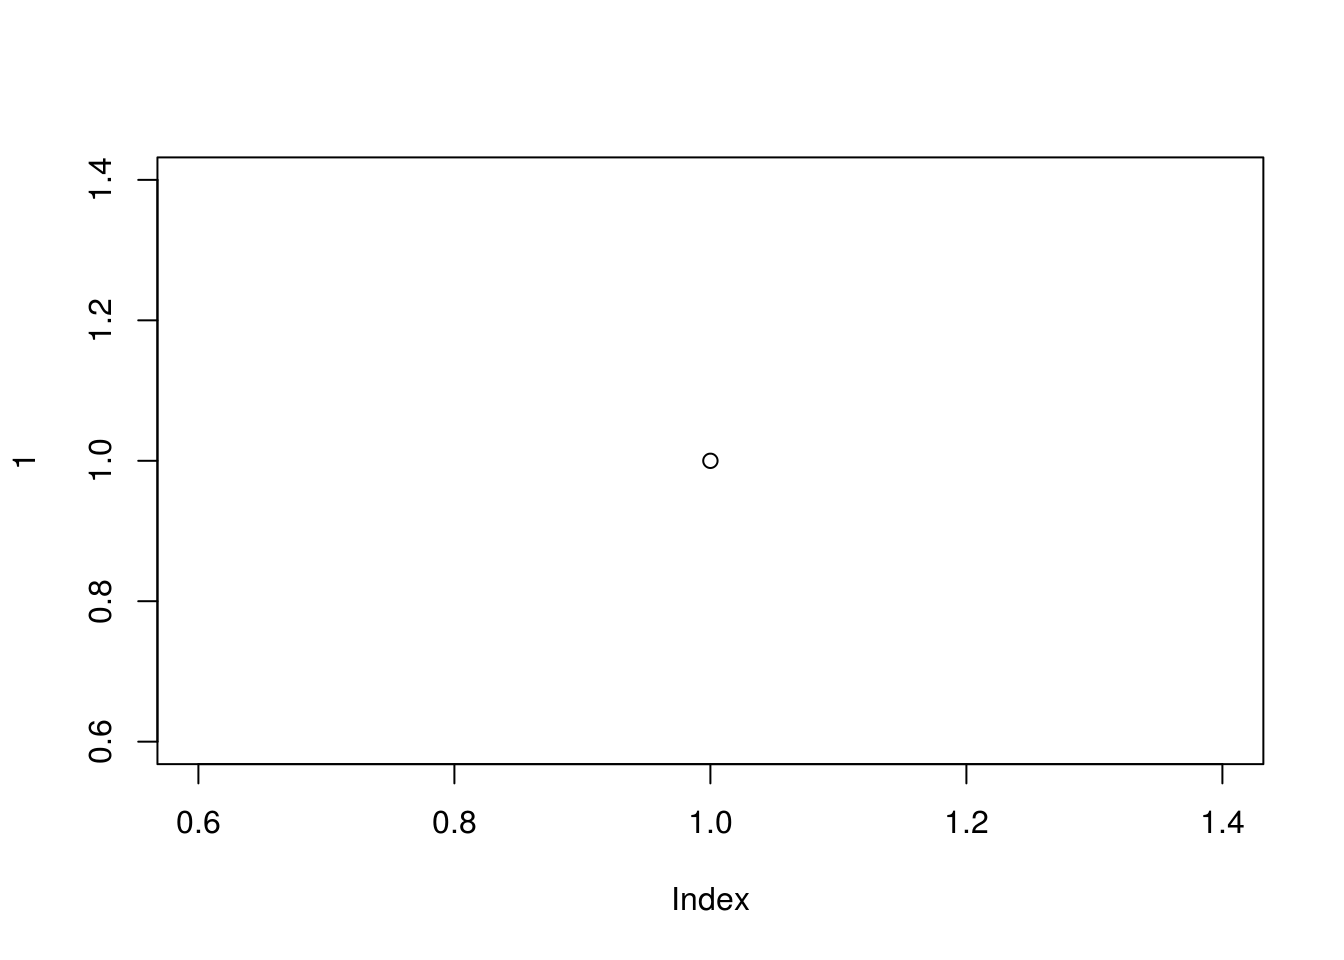
\includegraphics{brisbane-birds_files/figure-latex/unnamed-chunk-4-1.pdf}

\section{\texorpdfstring{Spiny-cheeked Honeyeater \emph{Acanthagenys
rufogularis}}{Spiny-cheeked Honeyeater Acanthagenys rufogularis}}\label{spiny-cheeked-honeyeater-acanthagenys-rufogularis}

\textbf{species level text in here}

\begin{figure}
\centering

\includegraphics{assets/missing.png}
\caption{No image for species}
\end{figure}

Lorem ipsum dolor sit amet, consectetur adipiscing elit. Donec sed justo
nunc. In in cursus turpis, sollicitudin pellentesque lacus. Aliquam et
orci malesuada, tristique justo quis, feugiat ex. Phasellus at sem sit
amet sapien consequat fringilla. Praesent pretium aliquet ante, eu
maximus augue placerat ut. Donec odio erat, vehicula non accumsan quis,
ultricies eu arcu. Aliquam erat volutpat.

In hac habitasse platea dictumst. Nullam lacus elit, luctus a cursus ut,
tempus id arcu. Quisque ornare eleifend augue, ac aliquet sapien posuere
porttitor. Nam lacinia, diam at molestie tempor, erat ligula vulputate
ligula, id rutrum magna justo in lorem. Vivamus posuere risus augue. Ut
velit elit, hendrerit sit amet lacus nec, mattis commodo neque. Cras vel
felis sed purus sollicitudin pharetra eu eget arcu. In volutpat eleifend
mauris, sed porta nunc dapibus a. Suspendisse fringilla tempus quam a
fermentum. Morbi quis lacus nec eros maximus interdum. Nullam venenatis
vehicula magna, a egestas est ornare vel. Fusce quis luctus orci, eget
congue dolor. Morbi luctus est justo, quis porttitor lacus facilisis sit
amet.

\begin{figure}
\includegraphics{brisbane-birds_files/figure-latex/unnamed-chunk-7-1} \caption{insert figure caption}\label{fig:unnamed-chunk-7}
\end{figure}

In ut elit facilisis, laoreet nulla et, porta leo. Vestibulum ante ipsum
primis in faucibus orci luctus et ultrices posuere cubilia Curae;
Phasellus ullamcorper eros at magna malesuada, ac maximus nibh
imperdiet. Pellentesque id purus nec erat pharetra iaculis. Mauris velit
neque, faucibus sed faucibus et, lobortis et felis. Morbi suscipit odio
pretium pellentesque finibus. Aenean ultrices ex sapien. Curabitur
tempus justo dolor, sit amet pulvinar diam fringilla at. Cras sit amet
auctor ante. Maecenas laoreet nisi sem, elementum condimentum sem
aliquam in. Praesent aliquam consequat leo sed fringilla. Aliquam sit
amet metus quis ligula ultricies pharetra ut vitae velit. Sed sed
vulputate mi. Nullam et elit vitae arcu efficitur venenatis.

\begin{figure}
\centering
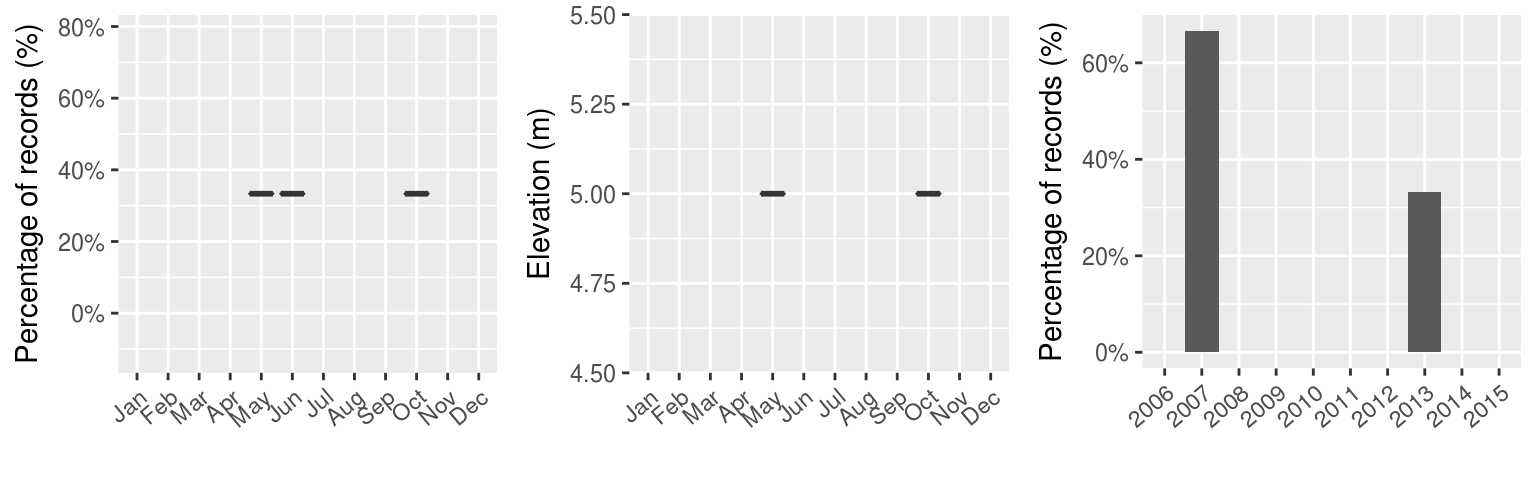
\includegraphics{brisbane-birds_files/figure-latex/unnamed-chunk-8-1.pdf}
\caption{\label{fig:unnamed-chunk-8}insert figure caption}
\end{figure}

\chapter{\texorpdfstring{Thornbills and Gerygones
\emph{Acanthizidae}}{Thornbills and Gerygones Acanthizidae}}\label{thornbills-and-gerygones-acanthizidae}

Lorem ipsum dolor sit amet, consectetur adipiscing elit. Donec sed justo
nunc. In in cursus turpis, sollicitudin pellentesque lacus. Aliquam et
orci malesuada, tristique justo quis, feugiat ex. Phasellus at sem sit
amet sapien consequat fringilla. Praesent pretium aliquet ante, eu
maximus augue placerat ut. Donec odio erat, vehicula non accumsan quis,
ultricies eu arcu. Aliquam erat volutpat.

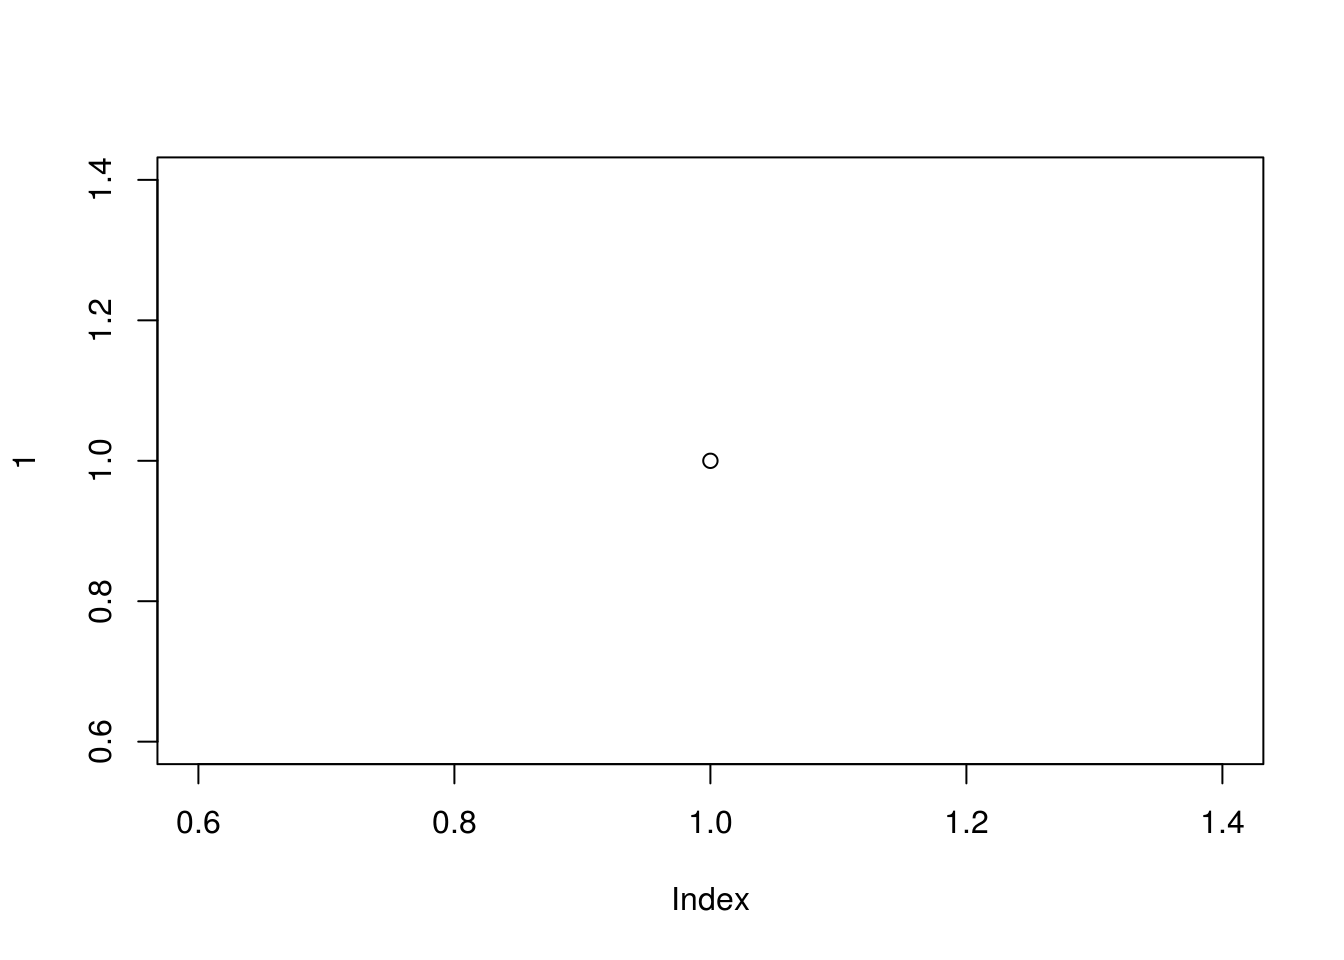
\includegraphics{brisbane-birds_files/figure-latex/unnamed-chunk-11-1.pdf}

\section{\texorpdfstring{Yellow-rumped Thornbill \emph{Acanthiza
chrysorrhoa}}{Yellow-rumped Thornbill Acanthiza chrysorrhoa}}\label{yellow-rumped-thornbill-acanthiza-chrysorrhoa}

\textbf{species level text in here}

\begin{figure}
\centering

\includegraphics{assets/missing.png}
\caption{No image for species}
\end{figure}

Lorem ipsum dolor sit amet, consectetur adipiscing elit. Donec sed justo
nunc. In in cursus turpis, sollicitudin pellentesque lacus. Aliquam et
orci malesuada, tristique justo quis, feugiat ex. Phasellus at sem sit
amet sapien consequat fringilla. Praesent pretium aliquet ante, eu
maximus augue placerat ut. Donec odio erat, vehicula non accumsan quis,
ultricies eu arcu. Aliquam erat volutpat.

In hac habitasse platea dictumst. Nullam lacus elit, luctus a cursus ut,
tempus id arcu. Quisque ornare eleifend augue, ac aliquet sapien posuere
porttitor. Nam lacinia, diam at molestie tempor, erat ligula vulputate
ligula, id rutrum magna justo in lorem. Vivamus posuere risus augue. Ut
velit elit, hendrerit sit amet lacus nec, mattis commodo neque. Cras vel
felis sed purus sollicitudin pharetra eu eget arcu. In volutpat eleifend
mauris, sed porta nunc dapibus a. Suspendisse fringilla tempus quam a
fermentum. Morbi quis lacus nec eros maximus interdum. Nullam venenatis
vehicula magna, a egestas est ornare vel. Fusce quis luctus orci, eget
congue dolor. Morbi luctus est justo, quis porttitor lacus facilisis sit
amet.

\begin{figure}
\includegraphics{brisbane-birds_files/figure-latex/unnamed-chunk-14-1} \caption{insert figure caption}\label{fig:unnamed-chunk-14}
\end{figure}

In ut elit facilisis, laoreet nulla et, porta leo. Vestibulum ante ipsum
primis in faucibus orci luctus et ultrices posuere cubilia Curae;
Phasellus ullamcorper eros at magna malesuada, ac maximus nibh
imperdiet. Pellentesque id purus nec erat pharetra iaculis. Mauris velit
neque, faucibus sed faucibus et, lobortis et felis. Morbi suscipit odio
pretium pellentesque finibus. Aenean ultrices ex sapien. Curabitur
tempus justo dolor, sit amet pulvinar diam fringilla at. Cras sit amet
auctor ante. Maecenas laoreet nisi sem, elementum condimentum sem
aliquam in. Praesent aliquam consequat leo sed fringilla. Aliquam sit
amet metus quis ligula ultricies pharetra ut vitae velit. Sed sed
vulputate mi. Nullam et elit vitae arcu efficitur venenatis.

\begin{figure}
\centering
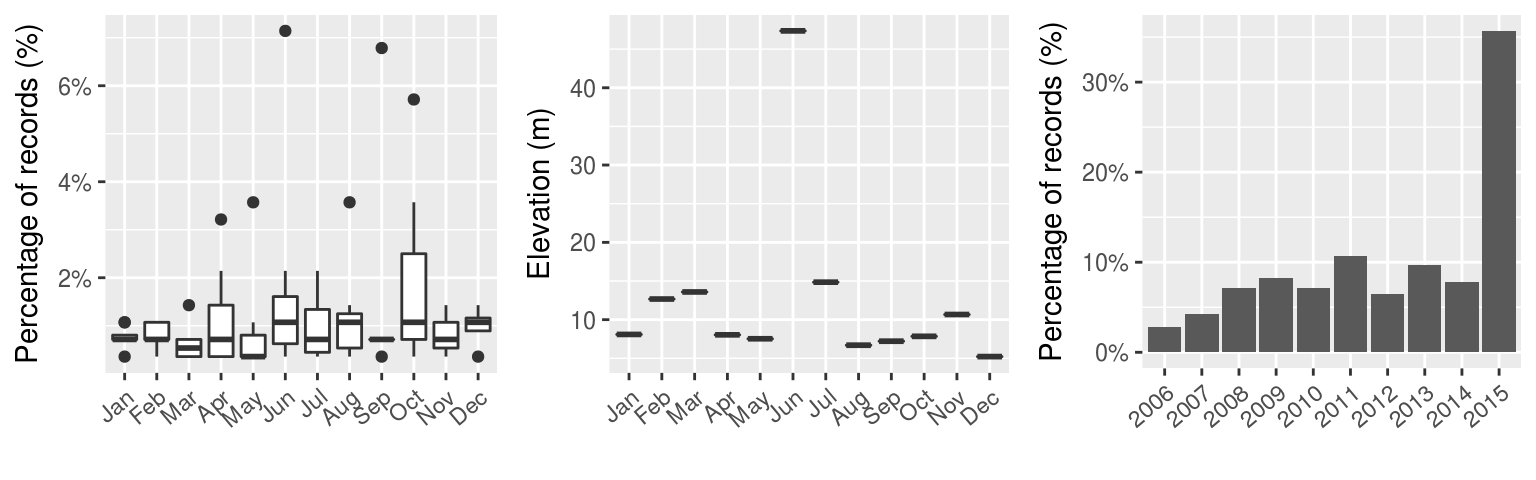
\includegraphics{brisbane-birds_files/figure-latex/unnamed-chunk-15-1.pdf}
\caption{\label{fig:unnamed-chunk-15}insert figure caption}
\end{figure}

\section{\texorpdfstring{Striated Thornbill \emph{Acanthiza
lineata}}{Striated Thornbill Acanthiza lineata}}\label{striated-thornbill-acanthiza-lineata}

\textbf{species level text in here}

\begin{figure}
\centering

\includegraphics{assets/missing.png}
\caption{No image for species}
\end{figure}

Lorem ipsum dolor sit amet, consectetur adipiscing elit. Donec sed justo
nunc. In in cursus turpis, sollicitudin pellentesque lacus. Aliquam et
orci malesuada, tristique justo quis, feugiat ex. Phasellus at sem sit
amet sapien consequat fringilla. Praesent pretium aliquet ante, eu
maximus augue placerat ut. Donec odio erat, vehicula non accumsan quis,
ultricies eu arcu. Aliquam erat volutpat.

In hac habitasse platea dictumst. Nullam lacus elit, luctus a cursus ut,
tempus id arcu. Quisque ornare eleifend augue, ac aliquet sapien posuere
porttitor. Nam lacinia, diam at molestie tempor, erat ligula vulputate
ligula, id rutrum magna justo in lorem. Vivamus posuere risus augue. Ut
velit elit, hendrerit sit amet lacus nec, mattis commodo neque. Cras vel
felis sed purus sollicitudin pharetra eu eget arcu. In volutpat eleifend
mauris, sed porta nunc dapibus a. Suspendisse fringilla tempus quam a
fermentum. Morbi quis lacus nec eros maximus interdum. Nullam venenatis
vehicula magna, a egestas est ornare vel. Fusce quis luctus orci, eget
congue dolor. Morbi luctus est justo, quis porttitor lacus facilisis sit
amet.

\begin{figure}
\includegraphics{brisbane-birds_files/figure-latex/unnamed-chunk-18-1} \caption{insert figure caption}\label{fig:unnamed-chunk-18}
\end{figure}

In ut elit facilisis, laoreet nulla et, porta leo. Vestibulum ante ipsum
primis in faucibus orci luctus et ultrices posuere cubilia Curae;
Phasellus ullamcorper eros at magna malesuada, ac maximus nibh
imperdiet. Pellentesque id purus nec erat pharetra iaculis. Mauris velit
neque, faucibus sed faucibus et, lobortis et felis. Morbi suscipit odio
pretium pellentesque finibus. Aenean ultrices ex sapien. Curabitur
tempus justo dolor, sit amet pulvinar diam fringilla at. Cras sit amet
auctor ante. Maecenas laoreet nisi sem, elementum condimentum sem
aliquam in. Praesent aliquam consequat leo sed fringilla. Aliquam sit
amet metus quis ligula ultricies pharetra ut vitae velit. Sed sed
vulputate mi. Nullam et elit vitae arcu efficitur venenatis.

\begin{figure}
\centering
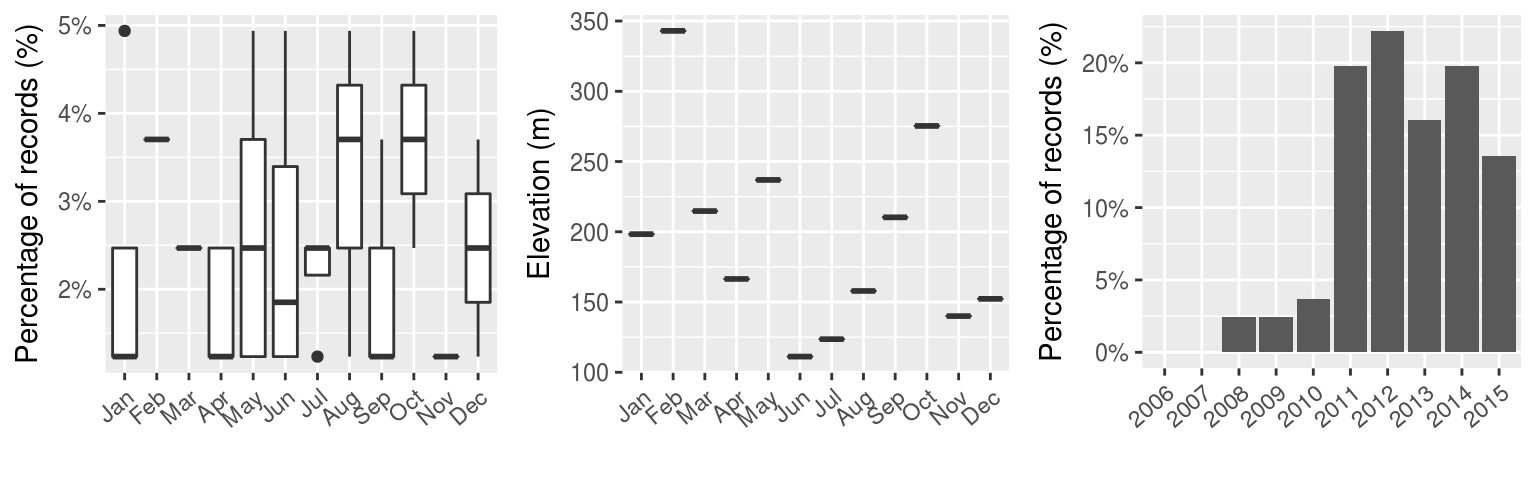
\includegraphics{brisbane-birds_files/figure-latex/unnamed-chunk-19-1.pdf}
\caption{\label{fig:unnamed-chunk-19}insert figure caption}
\end{figure}

\section{\texorpdfstring{Yellow Thornbill \emph{Acanthiza
nana}}{Yellow Thornbill Acanthiza nana}}\label{yellow-thornbill-acanthiza-nana}

\textbf{species level text in here}

\begin{figure}
\centering

\includegraphics{assets/missing.png}
\caption{No image for species}
\end{figure}

Lorem ipsum dolor sit amet, consectetur adipiscing elit. Donec sed justo
nunc. In in cursus turpis, sollicitudin pellentesque lacus. Aliquam et
orci malesuada, tristique justo quis, feugiat ex. Phasellus at sem sit
amet sapien consequat fringilla. Praesent pretium aliquet ante, eu
maximus augue placerat ut. Donec odio erat, vehicula non accumsan quis,
ultricies eu arcu. Aliquam erat volutpat.

In hac habitasse platea dictumst. Nullam lacus elit, luctus a cursus ut,
tempus id arcu. Quisque ornare eleifend augue, ac aliquet sapien posuere
porttitor. Nam lacinia, diam at molestie tempor, erat ligula vulputate
ligula, id rutrum magna justo in lorem. Vivamus posuere risus augue. Ut
velit elit, hendrerit sit amet lacus nec, mattis commodo neque. Cras vel
felis sed purus sollicitudin pharetra eu eget arcu. In volutpat eleifend
mauris, sed porta nunc dapibus a. Suspendisse fringilla tempus quam a
fermentum. Morbi quis lacus nec eros maximus interdum. Nullam venenatis
vehicula magna, a egestas est ornare vel. Fusce quis luctus orci, eget
congue dolor. Morbi luctus est justo, quis porttitor lacus facilisis sit
amet.

\begin{figure}
\includegraphics{brisbane-birds_files/figure-latex/unnamed-chunk-22-1} \caption{insert figure caption}\label{fig:unnamed-chunk-22}
\end{figure}

In ut elit facilisis, laoreet nulla et, porta leo. Vestibulum ante ipsum
primis in faucibus orci luctus et ultrices posuere cubilia Curae;
Phasellus ullamcorper eros at magna malesuada, ac maximus nibh
imperdiet. Pellentesque id purus nec erat pharetra iaculis. Mauris velit
neque, faucibus sed faucibus et, lobortis et felis. Morbi suscipit odio
pretium pellentesque finibus. Aenean ultrices ex sapien. Curabitur
tempus justo dolor, sit amet pulvinar diam fringilla at. Cras sit amet
auctor ante. Maecenas laoreet nisi sem, elementum condimentum sem
aliquam in. Praesent aliquam consequat leo sed fringilla. Aliquam sit
amet metus quis ligula ultricies pharetra ut vitae velit. Sed sed
vulputate mi. Nullam et elit vitae arcu efficitur venenatis.

\begin{figure}
\centering
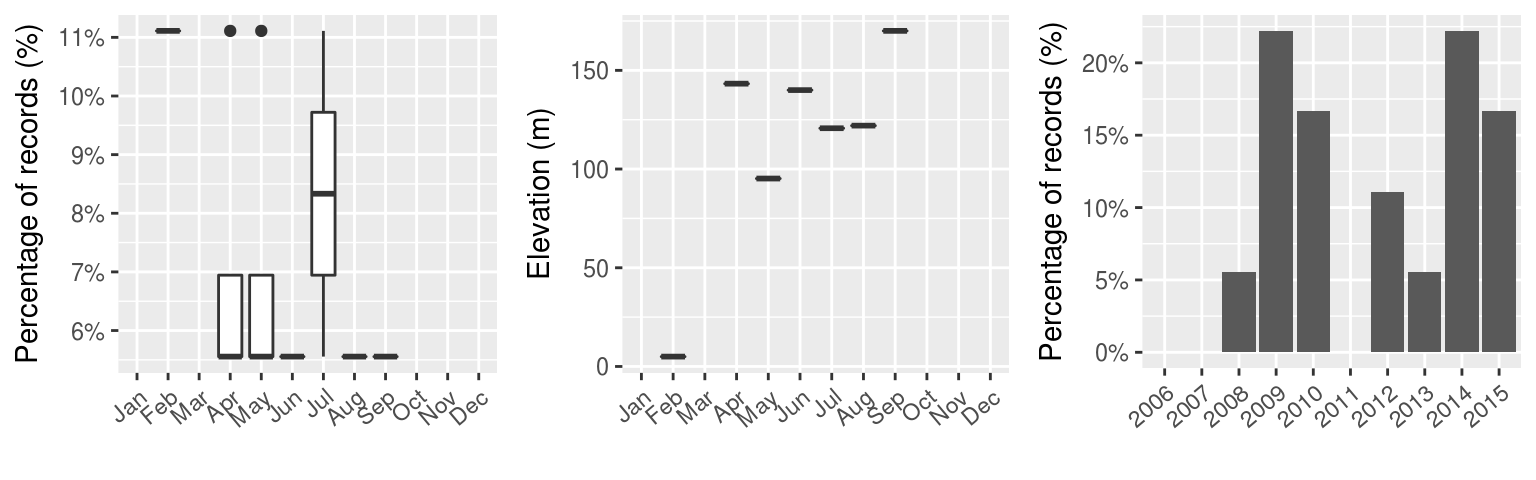
\includegraphics{brisbane-birds_files/figure-latex/unnamed-chunk-23-1.pdf}
\caption{\label{fig:unnamed-chunk-23}insert figure caption}
\end{figure}

\section{\texorpdfstring{Brown Thornbill \emph{Acanthiza
pusilla}}{Brown Thornbill Acanthiza pusilla}}\label{brown-thornbill-acanthiza-pusilla}

\textbf{species level text in here}

\begin{figure}
\centering

\includegraphics{assets/missing.png}
\caption{No image for species}
\end{figure}

Lorem ipsum dolor sit amet, consectetur adipiscing elit. Donec sed justo
nunc. In in cursus turpis, sollicitudin pellentesque lacus. Aliquam et
orci malesuada, tristique justo quis, feugiat ex. Phasellus at sem sit
amet sapien consequat fringilla. Praesent pretium aliquet ante, eu
maximus augue placerat ut. Donec odio erat, vehicula non accumsan quis,
ultricies eu arcu. Aliquam erat volutpat.

In hac habitasse platea dictumst. Nullam lacus elit, luctus a cursus ut,
tempus id arcu. Quisque ornare eleifend augue, ac aliquet sapien posuere
porttitor. Nam lacinia, diam at molestie tempor, erat ligula vulputate
ligula, id rutrum magna justo in lorem. Vivamus posuere risus augue. Ut
velit elit, hendrerit sit amet lacus nec, mattis commodo neque. Cras vel
felis sed purus sollicitudin pharetra eu eget arcu. In volutpat eleifend
mauris, sed porta nunc dapibus a. Suspendisse fringilla tempus quam a
fermentum. Morbi quis lacus nec eros maximus interdum. Nullam venenatis
vehicula magna, a egestas est ornare vel. Fusce quis luctus orci, eget
congue dolor. Morbi luctus est justo, quis porttitor lacus facilisis sit
amet.

\begin{figure}
\includegraphics{brisbane-birds_files/figure-latex/unnamed-chunk-26-1} \caption{insert figure caption}\label{fig:unnamed-chunk-26}
\end{figure}

In ut elit facilisis, laoreet nulla et, porta leo. Vestibulum ante ipsum
primis in faucibus orci luctus et ultrices posuere cubilia Curae;
Phasellus ullamcorper eros at magna malesuada, ac maximus nibh
imperdiet. Pellentesque id purus nec erat pharetra iaculis. Mauris velit
neque, faucibus sed faucibus et, lobortis et felis. Morbi suscipit odio
pretium pellentesque finibus. Aenean ultrices ex sapien. Curabitur
tempus justo dolor, sit amet pulvinar diam fringilla at. Cras sit amet
auctor ante. Maecenas laoreet nisi sem, elementum condimentum sem
aliquam in. Praesent aliquam consequat leo sed fringilla. Aliquam sit
amet metus quis ligula ultricies pharetra ut vitae velit. Sed sed
vulputate mi. Nullam et elit vitae arcu efficitur venenatis.

\begin{figure}
\centering
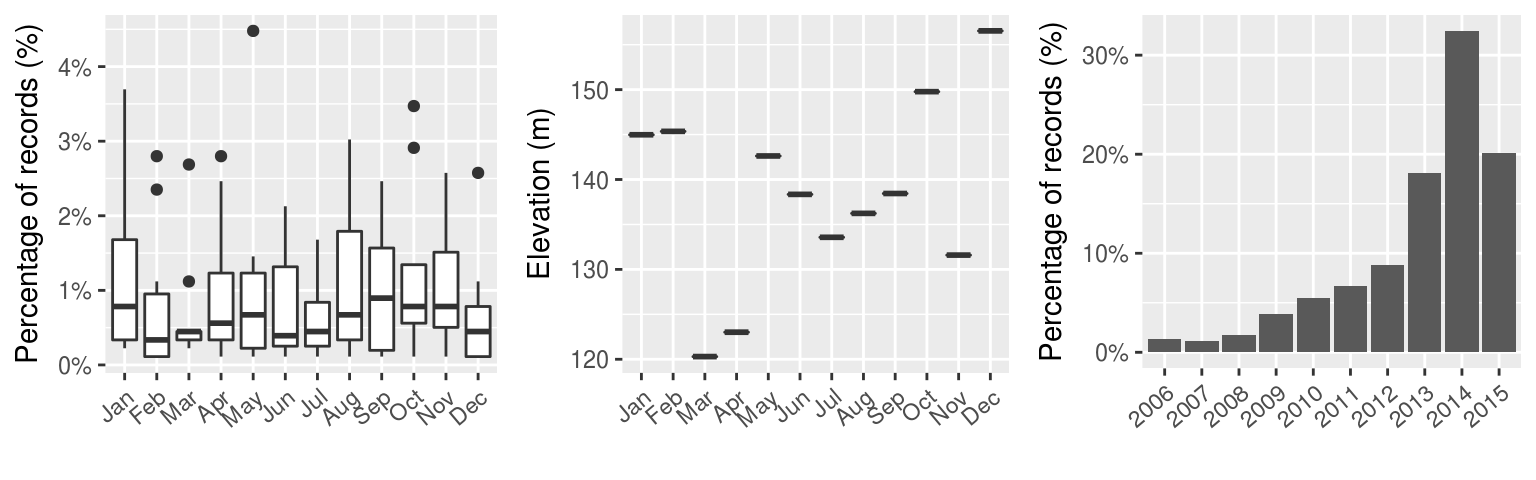
\includegraphics{brisbane-birds_files/figure-latex/unnamed-chunk-27-1.pdf}
\caption{\label{fig:unnamed-chunk-27}insert figure caption}
\end{figure}


\end{document}
